\section{Additional Safety Details}
\label{section:safetyappendix}


\subsection{Long-context Safety Mitigation Details} \label{app:lc_safety_mitigation}

\textbf{Supervised finetuning datasets.}
To mitigate many-shot jailbreaking risks (MSJ), we train our long-context models to respond in a safe manner, even when presented with demonstrations of unsafe behavior in context. We construct SFT datasets comprising $k$-shot examples, formatted as multi-turn dialogues, as follows:: 1 example = [ $k$ demonstrations | target query | target response ].

We extract target queries and responses from adversarial and borderline SFT datasets, maintaining a 1:2 ratio between the two. We create demonstration pairs (<prompt, response>) by following the protocol of \cite{anil2024many}, with both benign/borderline (B) and harmful (H) content, resulting in the following combinations: BB, BH, HB, HH.

We create three types of MSJ mitigation datasets:
\begin{itemize}
    \item \textit{Mixed:} Each example includes a mix of BB, BH, HB, and HH demonstration pairs in equal proportions within the context.
    \item \textit{Repeated }(\cite{anil2024many}'s strategy): Each example contains only one type of pair, with an equal proportion of BB/BH/HB/HH-only examples across the dataset.
    \item \textit{Combined: } The dataset is evenly split between "mixed" and "repeated" examples.
\end{itemize}
We also vary the maximum number of shots:
\begin{itemize}
    \item \textit{1 to 16 shots}: The dataset includes 1, 2, 4, 8, and 16-shot examples in equal proportions.
    \item \textit{1 to 128 shots}: The dataset includes 1, 2, 4, 8, 16, 32, 64, and 128-shot examples in equal proportions.
\end{itemize}
The combination of dataset type (mixed/repeated/combined) and maximum number of shots (1 to 16 / 1 to 128) yields six datasets for experimentation. Our baseline is a version of Llama 3 8B finetuned on a data mix that already includes a limited amount of short-context safety data. We train six 8B models, each by adding one of the MSJ mitigation datasets to the baseline data mix.

\textbf{Results.} Our mitigation strategies show a strong balance between safety and helpfulness, as evidenced by the performance on both safety and helpfulness benchmarks.

\textbf{Robustness to many-shot jailbreaking.}
We evaluate the effectiveness of our mitigation strategies against many-shot jailbreaking (MSJ) risks using our internal benchmark. As shown in Fig. \ref{fig:msj_ablation_results}, the baseline model is vulnerable to MSJ, with a violation rate (VR) that increases up to 31\% as the number of shots increases up to 256. In contrast, models finetuned on MSJ mitigation data exhibit significantly reduced VR.
Specifically, we observe the following:
\begin{itemize}
    \item 1 to 16 shots: Models trained on 1 to 16 shots MSJ mitigation data achieve a VR of 5\% for 16-shot attacks, an approximately 70\% reduction in VR. For attacks with > 16 shots, we observe a gradual increase as the number of shots increases, but VR remains below 13\% even for 256-shot attacks. 
    \item 1 to 128 shots: The model trained on \textit{1 to 128 shots, mixed} MSJ mitigation data maintains a VR consistently below 10\% even for 256-shot attacks, demonstrating more effective mitigation.
\end{itemize}
Note that \cite{anil2024many} suggest that finetuning is sufficient for mitigating MSJ in long context models with bounded context length but not for arbitrary context lengths.
Interestingly, our results suggest that our strategy of mixing BB, BH, HB, and HH demonstration pairs within the context is more effective than simply repeating these patterns (as in \cite{anil2024many}), when increasing the number of shots for the attack. This suggests that the model may benefit from learning to recognize and adapt to context switching. Next, we provide new insights into the impact of this mitigation strategy for MSJ on other important aspects of model performance, including long-context (LC) helpfulness, short-context (SC) safety and SC helpfulness.

\begin{figure}
    \centering
    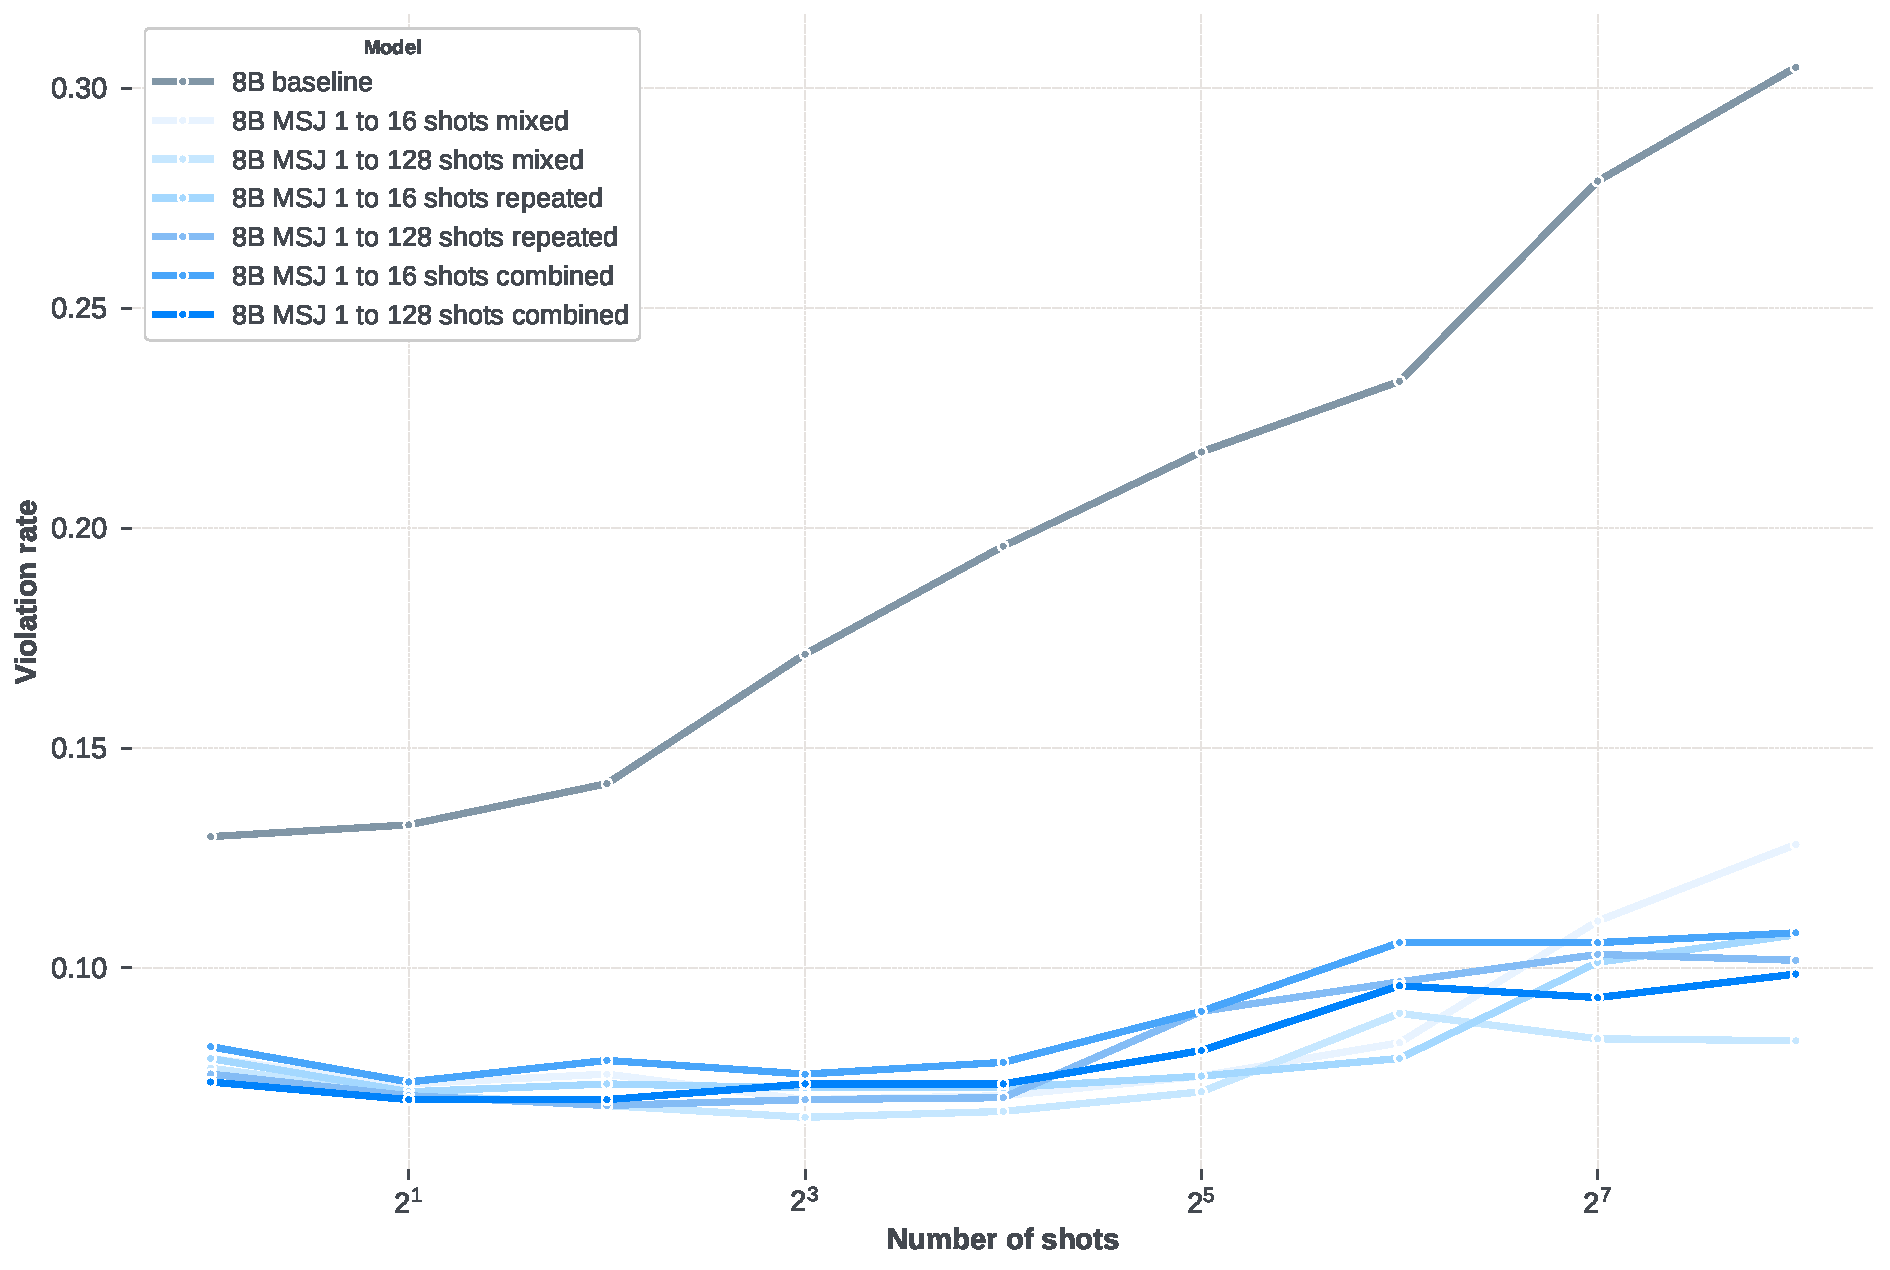
\includegraphics[width=0.8\linewidth]{appendices/lc_safety/figs/llama3_msj_ablations.pdf}
    \caption{Effectiveness of supervised finetuning against many-shot jailbreaking attack.}
    \label{fig:msj_ablation_results}
\end{figure}

\textbf{Long-context helpfulness.}
As shown in Table \ref{table:msj-lc-helpfulness}, we observe no significant impact of training on MSJ mitigation data in InfiniteBench, and notably, no regression was detected in LongbookQA and LongbookChoice.

On ZeroScrolls, we observe a drop on QuALITY (multiple-choice questions over long articles and stories) in most of our ablation experiments, except for the \textit{1 to 128 shots, repeated }MSJ mitigation dataset. We observe no regression on other ZeroScrolls subtasks.


\begin{table}[]
\begin{tabular}{@{}lllllll@{}}
\toprule
                                & \multicolumn{3}{l}{ZeroScrolls} & \multicolumn{2}{l}{InfiniteBench} & NIH          \\
                                & QuALITY  & SQuALITY  & Qasper  & LongbookQA    & LongbookChoice    & Multi-needle \\ \midrule
8B Baseline                     & 0.714     & 0.237     & 0.335   & 0.213         & 0.629             & 0.98         \\
8B MSJ 1 to 16, mixed     & 0.476     & 0.245     & 0.358   & 0.29          & 0.686             & 0.978        \\
8B MSJ 1 to 128, mixed    & 0.571     & 0.245     & 0.381   & 0.259              & 0.651                  & 0.981        \\
8B MSJ 1 to 16, repeated  & 0.429     & 0.249     & 0.458   & 0.271         & 0.655             & 0.975        \\
8B MSJ 1 to 128, repeated & 0.762     & 0.241     & 0.35    & 0.249         & 0.607             & 0.975        \\
8B MSJ 1 to 16, combined  & 0.619     & 0.237     & 0.346   & 0.256         & 0.677             & 0.973        \\
8B MSJ 1 to 128, combined & 0.619     & 0.238     & 0.4     & 0.299         & 0.624             & 0.969        \\ \bottomrule
\end{tabular}
\caption{Impact of MSJ mitigation on long-context helpfulness performance. \label{table:msj-lc-helpfulness}}
\end{table}

\textbf{Short-context safety.}
Using our internal SC safety benchmarks, we find that after supervised finetuning on MSJ mitigation data, the SC violation rate is greatly reduced with only a minor increase to the false refusal rate (Table \ref{table:msj-sc-safety}).





\begin{table}
\centering

\begin{tabular}{| l | l | l |}
\hline
 & \textbf{Violation Rate} & \textbf{False Refusal Rate} \\
\hline
8B Baseline  & 29.59\% & 1.91\% \\

8B MSJ 1 to 16 shots, mixed  & 12.79\% & 2.02\% \\

8B MSJ 1 to 128 shots, mixed & 13.24\% & 2.37\% \\

8B MSJ 1 to 16 shots, repeated  & 12.60\% & 2.16\% \\

8B MSJ 1 to 128 shots, repeated  & 13.52\% & 2.51\% \\

8B MSJ 1 to 16 shots, combined  & 14.61\% & 2.44\% \\

8B MSJ 1 to 128 shots, combined  & 14.06\% & 2.37\% \\
\hline

\end{tabular}
\caption{Impact of MSJ mitigation on short-context safety metrics. \label{table:msj-sc-safety}}
\end{table}



\textbf{Short-context helpfulness.}
We also evaluate the impact of our MSJ mitigation strategies on SC helpfulness using several public and internal benchmarks. Our results in Table \ref{table:msj-sc-helpfulness} show no degradation on academic benchmarks, including MMLU, except for a $\approx1.7\%$decrease on the MATH benchmark. Overall, mitigating MSJ via supervised finetuning does not significantly impact SC helpfulness performance.


\begin{table}[]
\begin{tabular}{@{}lllllll@{}}
\toprule
                                      & MMLU   & ARC-Challenge & GPQA   & HumanEval & GSM8K  & MATH   \\ \midrule
8B baseline & 69.2\% & 85.0\%        & 29.0\% & 64.0\%    & 81.9\% & 40.6\% \\
MSJ 1 to 16 shots, mixed              & 69.5\% & 84.8\%        & 28.6\% & 62.8\%    & 83.2\% & 38.9\% \\
MSJ 1 to 128 shots, mixed             & 69.3\% & 84.5\%        & 28.1\% & 64.6\%    & 82.2\% & 38.9\% \\
MSJ 1 to 16 shots, repeated           & 69.2\% & 84.6\%        & 29.2\% & 63.4\%    & 82.5\% & 39.4\% \\
MSJ 1 to 128 shots, repeated          & 69.2\% & 84.5\%        & 30.1\% & 61.6\%    & 81.8\% & 38.6\% \\
MSJ 1 to 16 shots, combined           & 69.1\% & 85.4\%        & 28.3\% & 64.0\%    & 82.4\% & 39.2\% \\
MSJ 1 to 128 shots, combined          & 69.0\% & 84.5\%        & 30.1\% & 64.6\%    & 82.9\% & 38.5\% \\ \bottomrule
\end{tabular}
\caption{Impact of MSJ mitigation on short-context helpfulness performance. \label{table:msj-sc-helpfulness}}
\end{table}


\subsection{Assigning safety labels to model responses for internal benchmarks}
\label{section:safety_labels}
\textbf{Human evals}

For each prompt in the benchmark set, we obtain a response from Llama 3 and competitor models. We send these prompt-response pairs to human annotators for review. Annotators review the safety of the response, the (potential) violation type, the refusal type, and the response tone. Each prompt-response pair is reviewed by three annotators, the results are aggregated with the majority label being assigned (e.g., a response labeled by two raters as unsafe and one as safe will be labeled as safe). A 5\% sample of the data is sent to policy experts for accuracy review, with high disagreement cases prioritized. That is, unanimously labeled items are under-sampled and cases where human reviewers disagreed on at least one label are over-sampled. Any examples which are labeled incorrectly are used to educate and calibration human annotators ensuring continued data quality improvements. Datasets used for violation and refusal rate comparisons obtained high expert-annotator agreement rates ($\geq 90\%$) on the accuracy review sample.

\textbf{AI-assisted evals}

During the development of Llama 3 AI-assisted annotations have been used to complement human annotations used to guide decision making. While human annotations are still considered the golden standard, AI-assisted annotations (a.k.a. the LLM-as-a-judge paradigm) are becoming increasingly popular to improve annotation scalability in terms of time and capacity, or budget. In this approach an LLM is used as a judge model to evaluate responses of another LLM (e.g., \cite{kim2024prometheus2opensource,chiang2023largelanguagemodelsalternative}). Examples where AI-assisted annotations were leveraged during the development of Llama 3 include ablation studies and model checkpoint evaluations.

Specifically, AI-assisted annotations were leveraged for two types of evaluations. The first evaluation assessed the violation rates of different content risk types across different model capabilities and languages. Here the judge is asked to assess whether a prompt-response pair violated any of the content risk policies. The second evaluation quantified false refusal prevalence, in which case the judge is asked whether the response is a refusal while the prompt set is scoped to questions which should not be refused, making any refusal therefore false.

The basis of our AI-assisted annotation systems were the Llama 3 checkpoints themselves at various model sizes (8B, 70B and 405B parameters). Different approaches are typically used to create judges from such base models. The simplest option is to use a few-shot in-context learning approach where assessment guidelines and policies, as well as examples of evaluations, are passed directly in the system prompt. An alternative approach is to first fine-tune models with annotated data to improve performance, and then apply it using a zero or few shot approach. Finally, different enhancement methods such as a jury of models (ensembling), prompt engineering or a hybrid human and AI-assisted setup, can still be explored to further boost performance. During Llama 3 development the AI-assisted methods were optimised for different types of evaluations.

Finally, it is crucial to assess the performance of AI-assisted annotations against human annotations. Different techniques have been proposed in literature and several studies propose an in-depth analysis of judge performance across different use cases (e.g., \cite{huang2024limitationsfinetunedjudgemodels, zheng2023judgingllmasajudgemtbenchchatbot}). We present a judge built to assess violation rate of content risk standard for English text capability as well as a judge to assess false refusal rate. Cohen Kappa was used as a quantitative measure of reliability of two raters rating the same thing, while correcting for how often the raters may agree by chance \cite{cohen1960}.

\begin{table}[h!]
\centering
\begin{tabular}{||c | c | c ||}
 \hline
 Task - Judge & Baseline & Hybrid setup \\
 \hline\hline
 English short context violation rate - Few Shot approach on Llama 3 405B & 0.59 & 0.90  \\
 English short context false refusal rate - Zero Shot approach on Llama 3 8B & 0.86 & -  \\
 \hline
\end{tabular}
\caption{Performance of AI-assisted annotations against human annotations golden dataset. Cohen Kappa metric. Hybrid setup refers to the case where judge predictions with low confidence are filtered and sent for human annotation (6.5\% humans, 93.5\% judge).}
\label{table:judge-performance}
\end{table}


In Table \ref{table:judge-performance} we observe that a zero shot judge based on Llama 3 8B model assessing false refusal achieves a Cohen Kappa of 0.88. This value is in the range of almost perfect agreement: hence this judge can be used to obtain an estimate of false refusal rate very close to human annotators.  Assessing violation rate appears to be a more complex task. Using a few shots approach based on Llama 405B for this task achieves a Cohen Kappa of 0.59 that is considered in the range of substantial agreement. Annotations obtained via this judge can be used to rank models, e.g., compare different model checkpoints or versions. We observe that using an hybrid human and AI-assisted setup, where judge predictions with low confidence are filtered and sent for human annotation, allows achieving a Cohen Kappa of 0.9, that is in the range of almost perfect agreement. This approach allows producing estimates of almost the same quality of fully human annotated samples with only 6.5\% of samples actually labelled by humans and the remaining 93.5\% by the judge.


\subsection{Additional Speech Safety Results}

Table~\ref{table:speech-safety-mutox-all} shows the detailed added and lost toxicity percentages across the 21 languages we evaluated on.



\providecommand{\bup}{($\boldsymbol\uparrow$)}
\providecommand{\bdown}{($\boldsymbol\downarrow$)}


\begin{table} 
\centering
\resizebox{\linewidth}{!}{
    \begin{tabular}{ l | c | c | c | c|c|c }
    \toprule
    \textbf{Language} & \textbf{Llama 3 8B AT \bdown} & \textbf{Llama 3 8B LT \bup} & \textbf{Llama 3 8B AT \bdown} & \textbf{Llama 3 8B LT \bup} & \textbf{AT Gemini \bdown} & \textbf{LT Gemini \bup} \\
    \midrule
    English & 0.84 & 15.09 & 0.68 & 15.46 & 1.44 & 13.42  \\
    Arabic & 2.40 & 4.45 & 2.82 & 4.47 & 1.12 & 6.95 \\
    Bengali & 0.54 & 2.45 & 0.42 & 2.42 & 0.52 & 2.55 \\
    Chinese & 0.60 & 8.40 & 0.47 & 8.55 & 1.07 & 8.30 \\
    German & 3.82 & 13.97 & 3.40 & 12.85 & 2.65 & 18.47 \\
    Greek & 3.52 & 6.67 & 2.22 & 7.00 & 2.60 & 7.12 \\
    Finnish & 4.90 & 8.12 & 4.15 & 8.70 & 2.90 & 8.22 \\
    French & 3.05 & 5.25 & 2.62 & 5.22 & 2.92 & 5.85 \\
    Hindi & 1.00 & 10.00 & 0.47 & 10.45 & 0.62 & 10.15 \\
    Hungarian & 4.05 & 10.67 & 3.77 & 10.40 & 1.84 & 10.25 \\
    Indonesian & 1.52 & 7.30 & 0.89 & 8.05 & 1.05 & 8.47 \\
    Italian & 4.12 & 9.37 & 3.45 & 9.72 & 3.12 & 10.10 \\
    Persian & 1.52 & 4.67 & 1.25 & 4.97 & 1.55 & 4.70 \\
    Polish & 5.92 & 6.10 & 5.97 & 6.10 & 3.87 & 7.55 \\
    Portuguese & 2.60 & 10.80 & 1.70 & 11.75 & 3.17 & 10.87 \\
    Russian & 3.32 & 6.10 & 3.80 & 5.94 & 2.42 & 8.00 \\
    Spanish & 2.81 & 12.49 & 2.35 & 13.64 & 3.52 & 12.86 \\
    Swahili & 0.70 & 5.40 & 0.77 & 5.32 & 0.65 & 5.37 \\
    Turkish & 2.00 & 4.85 & 1.95 & 4.77 & 0.75 & 6.37 \\
    Urdu & 0.52 & 17.67 & 0.60 & 17.52 & 0.54 & 17.97 \\
    Vietnamese & 2.72 & 6.77 & 2.07 & 8.77 & 1.52 & 10.92 \\
    \bottomrule
    \end{tabular}
}
    \caption{Speech toxicity of LLM output for different languages on MuTox dataset. AT refers to added toxicity (\%) and LT refers to lost toxicity (\%). \label{table:speech-safety-mutox-all}}
\end{table}
